%\documentclass[mathserif]{beamer}
\documentclass[handout]{beamer}
%\usetheme{Goettingen}
\usetheme{Warsaw}
%\usetheme{Singapore}
%\usetheme{Frankfurt}
%\usetheme{Copenhagen}
%\usetheme{Szeged}
%\usetheme{Montpellier}
%\usetheme{CambridgeUS}
%\usecolortheme{}
%\setbeamercovered{transparent}
\usepackage[english, activeacute]{babel}
\usepackage[utf8]{inputenc}
\usepackage{amsmath, amssymb}
\usepackage{dsfont}
\usepackage{graphics}
\usepackage{cases}
\usepackage{graphicx}
\usepackage{pgf}
\usepackage{epsfig}
\usepackage{amssymb}
\usepackage{multirow}	
\usepackage{amstext}
\usepackage[ruled,vlined,lined]{algorithm2e}
\usepackage{amsmath}
\usepackage{epic}
\usepackage{fontenc}
\usepackage{framed,color}
\usepackage{palatino, url, multicol}
\usepackage{listings}
%\algsetup{indent=2em}


\vspace{-0.5cm}
\title{Introduction to Bayesian Inference}
\vspace{-0.5cm}
\author[Felipe Bravo Márquez]{\footnotesize
%\author{\footnotesize  
 \textcolor[rgb]{0.00,0.00,1.00}{Felipe José Bravo Márquez}} 
\date{ \today }






\begin{document}
\begin{frame}
\titlepage


\end{frame}


%%%%%%%%%%%%%%%%%%%%%%%%%%%


\begin{frame}{Some Critics to the Frequentist Approach}
\scriptsize{
\begin{itemize}
 \item The statistical methods that we have discussed so far are known as frequentist (or classical) methods.
  \item The frequentist approach requires that all probabilities be defined by connection to the frequencies of events in very large samples. 
 \item This leads to frequentist uncertainty being premised on imaginary resampling of data. 
 \item If we were to repeat the measurement many many times, we would end up collecting a list of values that will have some pattern to it. 
 \item  It means also that parameters and models cannot have probability distributions, only measurements can.
 \item The distribution of these measurements is called a sampling distribution. 
 \item This resampling is never done, and in general it doesn't even make sense.
\end{itemize}

} 
\end{frame}

\begin{frame}{Bayesian Inference}
\scriptsize{
There is another approach to inference called Bayesian inference \cite{wasserman2013all}, which is based on the following postulates:
\begin{itemize}
 \item Probability describes \textbf{degree of belief}, not limiting frequency. 
 
 \begin{itemize}
 \scriptsize{
 \item  We can make probability statements about lots of things, not just data which are subject to random variation. 
 \item For example, I might say that "the probability that Albert Einstein drank a cup of tea on August 1, 1948" is .35. 
 \item This does not refer to any limiting frequency. 
 \item It reflects my strength of belief that the proposition is true.}
 \end{itemize}
 
 \item We can make probability statements about parameters, even though they are fixed constants.
 \item We make inferences about a parameter $\theta$ by producing a probability distribution for $\theta$. Inferences, such as point estimates and interval estimates, may then be extracted from this distribution.
\end{itemize}

} 
\end{frame}


\begin{frame}{Bayesian Inference}
\scriptsize{
\begin{itemize}
 \item In modest terms, Bayesian data analysis is no more than counting the numbers of ways
the data could happen, according to our assumptions \cite{mcelreath2020statistical}.
 \item In Bayesian analysis all alternative sequences of events that could have generated our data are evaluated.
 \item As we learn about what did happen, some of these alternative sequences are pruned. 
 \item In the end, what remains is only what is logically consistent with our knowledge \cite{mcelreath2020statistical}.
 \item Warning: understanding the essence of Bayesian inference can be hard.
 \item The following toy example tries to explain it in a gentle way.
\end{itemize}
 } 
\end{frame}


\begin{frame}{Counting Possibilities}
\scriptsize{
\begin{itemize}
 \item Suppose there's a bag, and it contains \textbf{four} marbles.
 \item These marbles come in two colors: \textbf{blue} and \textbf{white}. 
 \item We know there are four marbles in the bag, but we don't know how many are of each color. 
 \item We do know that there are five possibilities: 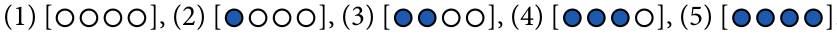
\includegraphics[scale=0.3]{pics/marbles1.png}
 \item These are the only possibilities consistent with what we know about the contents of the bag. Call these five possibilities the \textbf{conjectures}.
 \item Our goal is to figure out which of these conjectures is most \textbf{plausible}, given some \textbf{evidence} about the contents of the bag. 
 \item Evidence: A sequence of three marbles is pulled from the bag, one at a time, replacing the marble each time and shaking the bag, in that order. 
 \item The sequence that emerges is: 
\includegraphics[scale=0.5]{pics/marbles2.png}, which is our \textbf{data}. 
  
\end{itemize}
 } 
\end{frame}



\begin{frame}{Counting Possibilities}
\scriptsize{
\begin{itemize}
 \item Now, let's see how to use the data to infer what's in the bag.
 \item Let's begin by considering just the single conjecture, 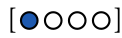
\includegraphics[scale=0.3]{pics/marbles3.png}, that the bag contains one blue and three white marbles. 
 \item On the first draw from the bag, one of four things could
happen, corresponding to one of four marbles in the bag.

\begin{figure}[h!]
	\centering
	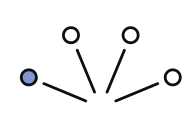
\includegraphics[scale=0.4]{pics/marbles4.png}
\end{figure}

\item Notice that even though the three white marbles look the same from a data perspective we just record the color of the marbles, after all they are really different events.

\item This is important, because it means that there are three more ways to see 
\includegraphics[scale=0.3]{pics/marbles5.png} than to see 
\includegraphics[scale=0.3]{pics/marbles6.png}.

\end{itemize}
 } 
\end{frame}



\begin{frame}{Counting Possibilities}
\scriptsize{
\begin{itemize}
 \item Now consider the garden as we get another draw from the bag. It expands the garden out one layer:

\begin{figure}[h!]
	\centering
	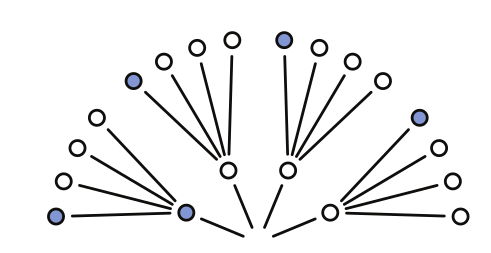
\includegraphics[scale=0.4]{pics/marbles7.png}
\end{figure}

\item Now there are 16 possible paths through the garden, one for each pair of draws.

%\item On the second draw from the bag, each of the paths above again forks into four possible paths. Why?

\end{itemize}
 } 
\end{frame}


\begin{frame}{Counting Possibilities}
\scriptsize{
\begin{itemize}
 %\item Because we believe that our shaking of the bag gives each marble a fair chance at being drawn, regardless of which marble was drawn previously. 
 \item The third layer is built in the same way, and the full garden is shown
 below:
\begin{figure}[h!]
	\centering
	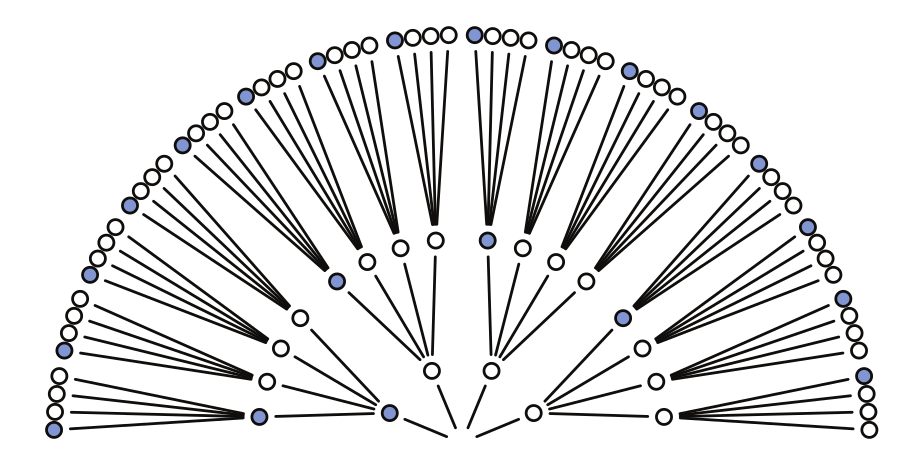
\includegraphics[scale=0.3]{pics/marbles8.png}
\end{figure}

\item There are $4^3 = 64$ possible paths in total.

\end{itemize}
 } 
\end{frame}


\begin{frame}{Counting Possibilities}
\scriptsize{
\begin{itemize}
 \item As we consider each draw from the bag to get 
\includegraphics[scale=0.5]{pics/marbles2.png}, some of these paths are logically eliminated.
 \item The first draw tuned out to be 
\includegraphics[scale=0.3]{pics/marbles6.png}, recall, so the three white paths at the bottom are eliminated right away. 
 \item If you imagine the real data tracing out a path, it must have passed through the one blue path near the origin. 
 \item The second draw from the bag produces 
\includegraphics[scale=0.3]{pics/marbles5.png}, so three of the paths forking out of the first blue marble remain.
 \end{itemize}
 } 
\end{frame}


\begin{frame}{Counting Possibilities}
\scriptsize{
\begin{itemize}
 \item As the data trace out a path, we know it must have passed through one of those three white paths (after the first blue path).
 \item But we don't know which one, because we recorded only the color of each marble.
 \item Finally, the third draw is 
\includegraphics[scale=0.3]{pics/marbles6.png}. 
 \item Each of the remaining three paths in the middle layer sustain one blue path, leaving a total of three ways for the sequence 
\includegraphics[scale=0.3]{pics/marbles2.png} to appear, assuming the bag contains 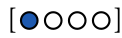
\includegraphics[scale=0.3]{pics/marbles3.png}.
\end{itemize}
 } 
\end{frame}


\begin{frame}{Counting Possibilities}
\scriptsize{
\begin{itemize}
 \item The figure below shows the forking paths again, now with logically eliminated paths grayed out.

\begin{figure}[h!]
	\centering
	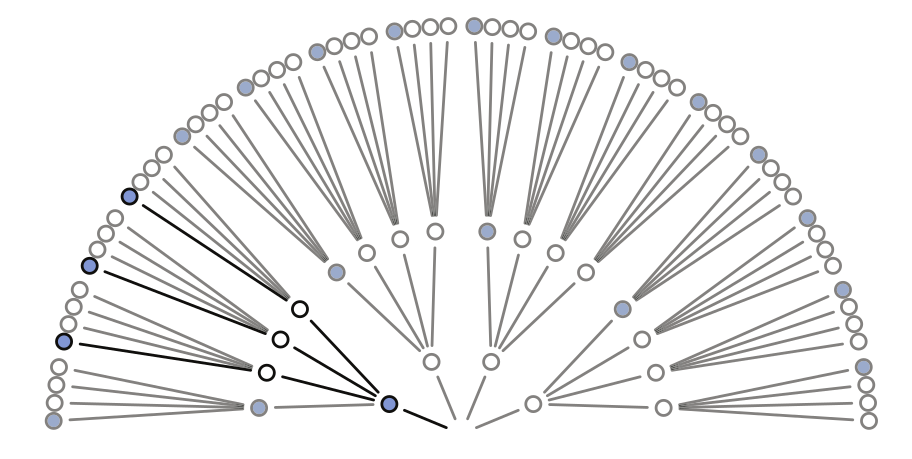
\includegraphics[scale=0.33]{pics/marbles9.png}
\end{figure}
\end{itemize}
 } 
\end{frame}



\begin{frame}{Counting Possibilities}
\scriptsize{
\begin{itemize}
\item We can't be sure which of those three paths the actual data took.
\item But as long as we're considering only the possibility that the bag contains one blue and three white marbles, we can be sure that the data took one of those three paths.

\item Those are the only paths consistent with both our knowledge of the bag's contents (four marbles, white or blue) and the data (
\includegraphics[scale=0.3]{pics/marbles2.png}).  

 \item This demonstrates that there are three (out of 64) ways for a bag containing 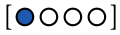
\includegraphics[scale=0.3]{pics/marbles17.png} to produce the data.
 \item We have no way to decide among these three ways. 
\end{itemize}
 } 
\end{frame}


\begin{frame}{Counting Possibilities}
\scriptsize{
\begin{itemize}
 \item The inferential power comes from comparing this count to the numbers of ways each of the other conjectures of the bag's contents could produce the same data. 
 \item For example, consider the conjecture 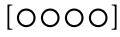
\includegraphics[scale=0.3]{pics/marbles10.png}. 
 \item There are zero ways for this conjecture to produce the observed data, because even one 
\includegraphics[scale=0.3]{pics/marbles6.png} is logically incompatible with it. 
\item The conjecture 
\includegraphics[scale=0.3]{pics/marbles11.png} is likewise logically incompatible with the data. 
\item So we can eliminate these two conjectures, because neither provides even a single path that is consistent with the data.
\item The next slide's figure displays all the paths for the remaining three conjectures: 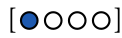
\includegraphics[scale=0.3]{pics/marbles3.png}, 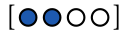
\includegraphics[scale=0.3]{pics/marbles13.png}, and 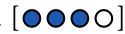
\includegraphics[scale=0.3]{pics/marbles14.png}.

\end{itemize}
 } 
\end{frame}




\begin{frame}{Counting Possibilities}
\scriptsize{
\begin{figure}[h!]
	\centering
	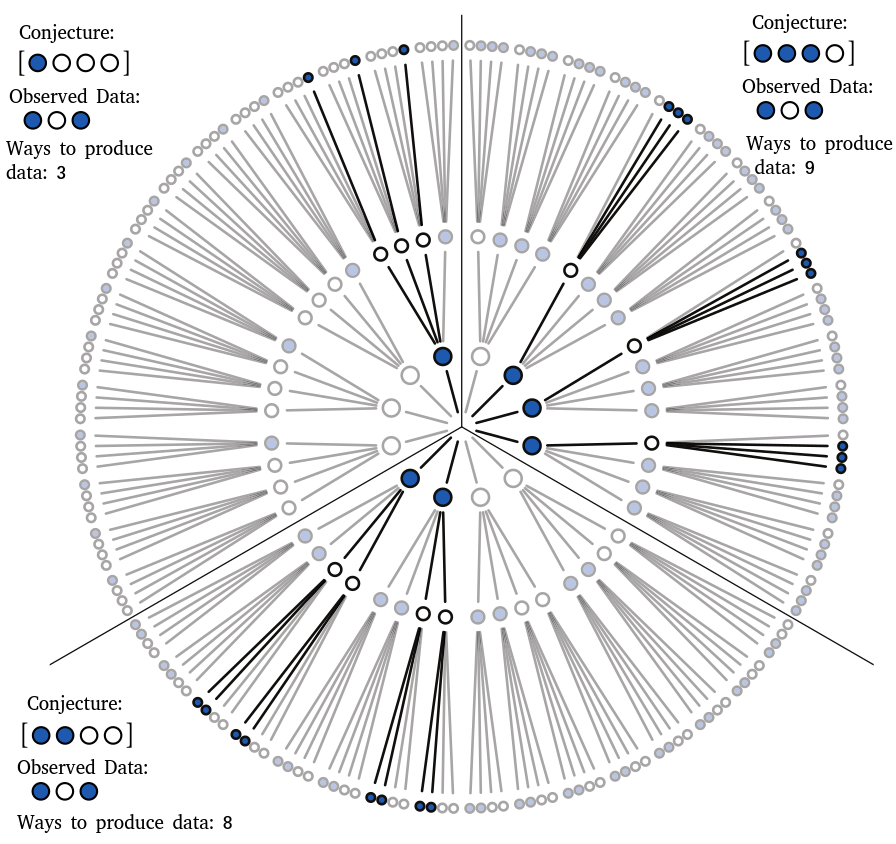
\includegraphics[scale=0.35]{pics/marbles12.png}
\end{figure}
 } 
\end{frame}

\begin{frame}{Counting Possibilities}
\scriptsize{
\begin{itemize}
 \item The number of ways to produce the data, for each conjecture, can be computed by first counting the number of paths in each ``ring'' of the garden and then by multiplying these counts together.
 \begin{figure}[h!]
	\centering
	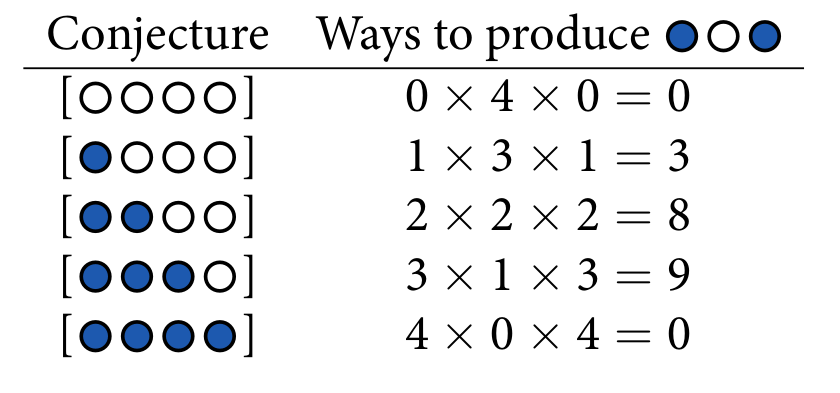
\includegraphics[scale=0.3]{pics/marbles15.png}
\end{figure}
\item By comparing these counts, we have part a way to rate the relative \textbf{plausibility} of each conjectured bag composition.
\end{itemize}
 } 
\end{frame}

\begin{frame}{Combining other information}
\scriptsize{
\begin{itemize}
 \item We may have additional information about the relative plausibility of each conjecture. 
 \item This information could arise from knowledge of how the contents of the bag were generated. 
 \item It could also arise from previous data. 
 \item Whatever the source, it would help to have a way to combine different sources of information to update the plausibilities. 
 \item Luckily there is a natural solution: Just multiply the counts.
\end{itemize}
 } 
\end{frame}


\begin{frame}{Combining other information}
\scriptsize{
\begin{itemize}
 \item Suppose that each conjecture is equally plausible at the start.
 \item So we just compare the counts of ways in which each conjecture is compatible with the observed data: 
\includegraphics[scale=0.3]{pics/marbles2.png}.
 \item This comparison suggests that 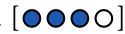
\includegraphics[scale=0.3]{pics/marbles14.png} is slightly more plausible than 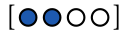
\includegraphics[scale=0.3]{pics/marbles13.png}, and both are about three times more plausible than 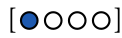
\includegraphics[scale=0.3]{pics/marbles3.png}. 
\item Since these are our initial counts, and we are going to update them next, let's label them \textbf{prior}.
\item Now suppose we draw another marble from the bag to get another observation: 
\includegraphics[scale=0.3]{pics/marbles6.png}. 
\item How can we update our plausibilities about each conjecture based on this new evidence?
\item There are two choices discussed next. 
\end{itemize}
 } 
\end{frame}


\begin{frame}{Combining other information}
\scriptsize{
\begin{itemize}
 \item Option 1: draw a forking path with four layers and do the counting again.
\item Option 2: Update previous counts (0, 3, 8, 9, 0) with the new information by multiplying the new count by the old count.
\item Both approach are mathematically identical as long
as the new observation is logically independent of the previous observations. 

\begin{figure}[h!]
	\centering
	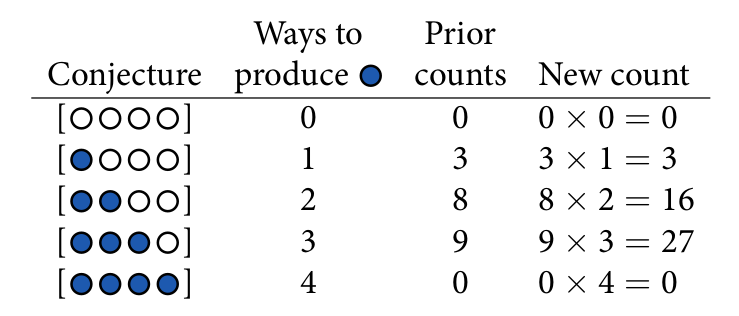
\includegraphics[scale=0.33]{pics/marbles16.png}
\end{figure}
\end{itemize}
 } 
\end{frame}



\begin{frame}{Combining other information}
\scriptsize{
\begin{itemize}
 \item In the previous example, the prior data and new data are of the same type: marbles drawn from the bag. 
 \item But in general, the prior data and new data can be of different types. 
 \item Suppose for example that someone from the marble factory tells you that blue marbles are rare.
 \item So for every bag containing 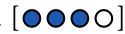
\includegraphics[scale=0.3]{pics/marbles14.png}, they made two bags containing 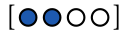
\includegraphics[scale=0.3]{pics/marbles13.png} and three bags containing 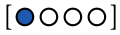
\includegraphics[scale=0.3]{pics/marbles17.png} . 
 \item They also ensured that every bag contained at least one blue and one white marble. 
\end{itemize}
 } 
\end{frame}


\begin{frame}{Combining other information}
\scriptsize{
\begin{itemize}
 \item We can update our counts again:
\begin{figure}[h!]
	\centering
	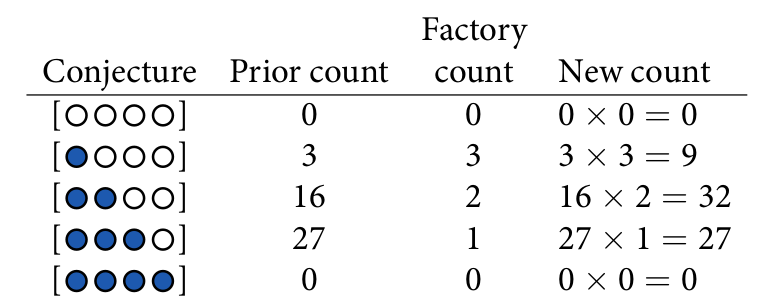
\includegraphics[scale=0.33]{pics/marbles18.png}
\end{figure}
\item Now the conjecture 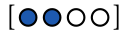
\includegraphics[scale=0.3]{pics/marbles13.png} is most plausible, but barely better than 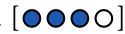
\includegraphics[scale=0.3]{pics/marbles14.png}.
\item Is there a threshold difference in these counts at which we can safely decide that one of the conjectures is the correct one? 
\item We will explore this question next.
\end{itemize}
 } 
\end{frame}

\begin{frame}{From counts to probability}
\scriptsize{
\begin{itemize}
 \item  So far, we have defined the updated plausibility of each possible composition of the bag, after seeing the data, as:
 \begin{figure}[h!]
	\centering
	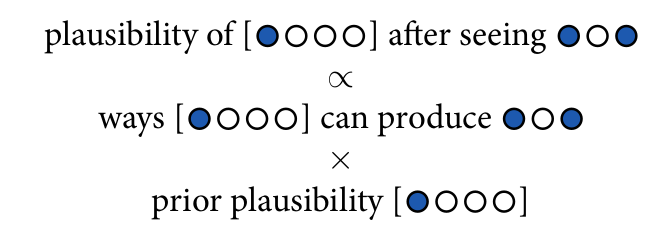
\includegraphics[scale=0.3]{pics/marbles19.png}
\end{figure}
\item The problem of representing plausibilities as counts is that these numbers grow very quickly  as  the amount of data grows. 
 \item It is better to standardize them to turn them into probabilities.
\end{itemize}
 } 
\end{frame}


\begin{frame}{From counts to probability}
\scriptsize{
\begin{itemize}
 \item Now  we will formalize the Bayesian framework using probabilities.
\item Let index our conjecture with a parameter $\theta$ defined as the fractions of marbles from the bag that are blue:

$\theta=0 \rightarrow$ 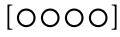
\includegraphics[scale=0.3]{pics/marbles10.png}, $\theta=0.25 \rightarrow$ 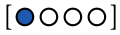
\includegraphics[scale=0.3]{pics/marbles17.png}, $\theta=0.5 \rightarrow$ 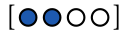
\includegraphics[scale=0.3]{pics/marbles13.png},  $\theta=0.75 \rightarrow$ 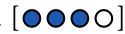
\includegraphics[scale=0.3]{pics/marbles14.png}, $\theta=1 \rightarrow$ 
\includegraphics[scale=0.3]{pics/marbles11.png}.

\item Let's call our data 
\includegraphics[scale=0.3]{pics/marbles2.png} $d$. 

\item We construct probabilities by standardizing the plausibility so that the sum of the plausibilities for all possible conjectures will be one.

\begin{equation}
 \text{plausibility of $\theta$ after $d$} = \frac{\text{ways $\theta$ can produce $d$} \times \text{prior plausibility $\theta$}}{\text{sum of products}}
\end{equation}

\item This is essentially the Bayes theorem:

\begin{equation}
 \mathbb{P}(\theta|d) = \frac{\mathbb{P}(d|\theta) \times \mathbb{P}(\theta)}{\mathbb{P}(d)}
\end{equation}


\end{itemize}
 } 
 
 \end{frame}



\begin{frame}{From counts to probability}
\scriptsize{
\begin{itemize}
\item The denominator $\mathbb{P}(d)$ (that standardizes values to sum one) can be expressed by the law of total probabilities as: 
\begin{equation}
 \mathbb{P}(d) =  \sum_\theta \mathbb{P}(d|\theta) \times \mathbb{P}(\theta) 
\end{equation}

 \item Let's consider the prior assumptions that all conjectures are equally plausible at the start, then $\mathbb{P}(\theta)$ is uniformly distributed.  \\ 
 
 \vspace{0.3cm}
  \begin{tabular}{c|c|c|c|c} \hline
$\theta$ & $\mathbb{P}(\theta)$ & Ways to Produce Data & $\mathbb{P}(d|\theta)$ & $\mathbb{P}(\theta|d) = \mathbb{P}(d|\theta)*\mathbb{P}(\theta) / \mathbb{P}(d)$  \\ \hline
0 & 1/5 & 0 & 0/64 &  $\frac{0/64*1/5}{0.0625}$ =0 \\
0.25 & 1/5 & 3 & 3/64 & $\frac{3/64*1/5}{0.0625}$ = 0.15
\\
0.5 & 1/5 & 8 & 8/64 & $\frac{8/64*1/5}{0.0625}$ = 0.4 \\
0.75 & 1/5 & 9 & 9/64 & $\frac{9/64*1/5}{0.0625}$ = 0.45 \\
1 & 1/5 & 0 & 0/64 & $\frac{0/64*1/5}{0.0625}$ = 0 \\ 
\end{tabular} 
\vspace{0.3cm} 
 
\item where $\mathbb{P}(d)$ = 1/5 * 0/64 + 1/5*3/64 + 1/5*8/64+1/5*9/64+1/5*0/64 = 0.0625 
 
 
\end{itemize}
 } 
 

\end{frame}


\begin{frame}{From counts to probability}
\scriptsize{
\begin{itemize}
\item Let's use the factory counts information (blue marbles are rare) now in our prior assumptions of $\mathbb{P}(\theta)$.  \\ 
\item This can be done by normalizing the factory counts.  

\item Notice that this new prior assumption doesn't affect the ways each conjecture can generate the data and $\mathbb{P}(d|\theta)$ remains unchanged.
 
 \vspace{0.3cm}
  \begin{tabular}{c|c|c|c|c} \hline
$\theta$ & Factory count & $\mathbb{P}(\theta)$ &  $\mathbb{P}(d|\theta)$ & $\mathbb{P}(\theta|d) = \mathbb{P}(d|\theta)*\mathbb{P}(\theta) / \mathbb{P}(d)$  \\ \hline
0 & 0 & 0/6 &  0/64 &  $\frac{0/64*0/6}{0.08854167}$ =0 \\
0.25 & 3 & 3/6 & 3/64 & $\frac{3/64*3/6}{0.08854167}$ = 0.2647059
\\
0.5 & 2 & 2/6  & 8/64 & $\frac{8/64*2/6}{0.08854167}$ = 0.4705882 \\
0.75 & 1 &  1/6 & 9/64 & $\frac{9/64*1/6}{0.08854167}$ = 0.2647059  \\
1 &  0 & 0/6 &  0/64 & $\frac{0/64*0/6}{0.08854167}$ = 0 \\ 
\end{tabular} 
\vspace{0.3cm} 
 
\item where $\mathbb{P}(d)$= 0/6 * 0/64 + 3/6*3/64 + 2/6*8/64+1/6*9/64+0/6*0/64 =  0.08854167

\item Two different prior assumptions led us to different values of $\mathbb{P}(\theta|d)$.
 
\end{itemize}
 } 

\end{frame}


\begin{frame}{From counts to probability}
\scriptsize{
\begin{figure}[h!]
	\centering
	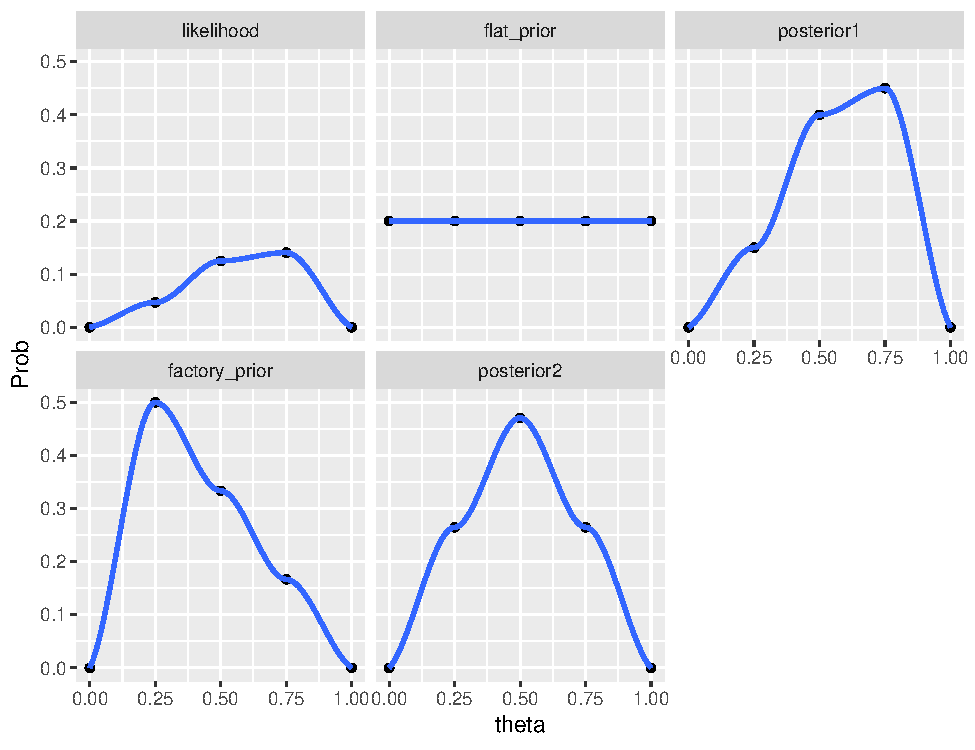
\includegraphics[scale=0.63]{pics/marbles_dist.pdf}
\end{figure}
 } 
 

\end{frame}


\begin{frame}{Bayesian Components}
\scriptsize{
Now we will introduce the names of the components of our Bayesian model. \\


\begin{block}{Density and Mass functions}
Because the Bayesian framework applies to both discrete and continuous random variables, we will use function $f$ (instead of $\mathbb{P}$) to refer to both probability mass and density functions.
\end{block}

\begin{itemize}
\item \textbf{Parameter} $\theta$:  A way of indexing possible explanations of the data. In our example $\theta$ is a conjectured proportion of blue marbles. 

\item \textbf{Likelihood} $f(d|\theta)$: The relative number of ways that a value $\theta$ can produce the data. It is derived by enumerating all the possible data sequences that could have happened and then eliminating those sequences inconsistent with the data.
\item \textbf{Prior probability} $f(\theta)$: The prior plausibility of any specific value of $\theta$.
 
\item \textbf{Posterior probability} $f(\theta|d)$: The new, updated plausibility of any specific $\theta$. 

\item \textbf{Evidence} or \textbf{Average Likelihood} $f(d)$: the average probability of the data averaged over the prior. It’s job is just to standardize the posterior, to ensure it sums (integrates) to one. 
 
\end{itemize}
 } 

 
 
 
\end{frame}


\begin{frame}{Bayesian Components}
\scriptsize{
\begin{itemize}

\item It is important to remark that in the Bayesian setting a parameter $\theta$ is random a variable, so we can make probability statements about it.

\item Whereas in the frequentist approach parameters are considered unknown quantities. 

\item This is an important property of Bayesian inference: despite $\theta$ is an \textbf{unobseved variable} we can treat is a random variable and calculate $f(\theta)$ or $f(\theta|d)$.

\item The likelihood function  $f(d|\theta)$ is very similar to the likelihood function in the frequentist approach $f(d;\theta)$ but now we can condition on $\theta$ instead of just using it as function parameter.

\item All the probability functions of a Bayesian model can correspond to either 1) a probability mass or 2) a density functions depending if the variable (observed or unobserved) is discrete or continuous.

\end{itemize}
 } 

\end{frame}


\begin{frame}{Bayesian Components}
\scriptsize{
\begin{itemize}

\item The general equation that relates all Bayesian components (for both density and mass functions) is the following:

\begin{equation}
 f(\theta|d) = \frac{f(d|\theta) \times f(\theta)}{f(d)}
\end{equation}

\item This equation is essentially the Bayes theorem (for both density and mass functions).

\item It says that the probability of any particular value of $\theta$ considering the data $d$, is proportional to the product of the relative plausibility of the data, conditional on $\theta$, and the prior plausibility of $\theta$.

\item This product is then divided by the average probability of the data to produce a valid probability distribution for the posterior (to sum or integrate to one).

\item We must bear in mind that Bayesian statistics is not only about using Bayes theorem. 

\item There are many non-Bayesian techniques that use this theorem.

\item Bayesian inference uses the Bayes theorem more generally, to quantify uncertainty about unobserved variables such as parameters.
\end{itemize}
 } 

\end{frame}




\begin{frame}{Bayesian Components}
\scriptsize{
\begin{itemize}

\item In the marble example $\theta$ is discrete so the prior and the posterior are probability mass functions.

\item When $\theta$ is continous, the prior and the posterior are density functions, and the \textbf{evidence} or \textbf{average likelihood} is calculated with an integral called \textbf{marginal}

\begin{equation}
 f(d) = \int_{\theta}f(d|\theta)f(\theta)d\theta  
\end{equation}

\item In most cases this integral doesn't have a closed solution.

\item However, there are nice computational methods available that can efficiently approximate the posterior even when the evidence cannot be calculated (e.g., MCMC, Variational Inference). 

\item Next, we will go deeper into these concepts by building another Bayesian toy model.
 
\end{itemize}
 } 

\end{frame}



\begin{frame}{A Globe Model}
\scriptsize{
\begin{itemize}

\item We have a globe representing our planet. 
\item We want to estimate much of the surface is covered in water. 
\item We adopt the following strategy: we toss the globe up in the air, we catch it, record whether or not the surface under your right index finger is water or
land. 
\item Then we toss the globe up in the air again and repeat the procedure.
\item The first nine samples are:
W L W W W L W L W
where W indicates water and L indicates land.
\item We observed 6 W and 3 L. This is our data.
\end{itemize}
 } 
 
\scriptsize{
\begin{figure}[h!]
	\centering
	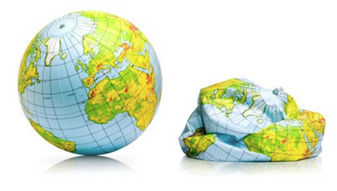
\includegraphics[scale=0.4]{pics/globe.png}
\end{figure}
 }  

\end{frame}

\begin{frame}{A Globe Model}
Designing a simple Bayesian model benefits from a design loop with three steps.
\begin{enumerate}
 \item Data story: Motivate the model by narrating how the data might arise.
\item Update: Educate your model by feeding it the data.
\item Evaluate: All statistical models require supervision, leading to model revision. \footnote{We won't elaborate on this part until later in the course..}
\end{enumerate}

\end{frame}



\begin{frame}{Data Story}
\scriptsize{
\begin{itemize}
\item You can motivate your data story by trying to explain how each piece of data is born. 
\item This usually means describing aspects of the underlying reality as well as the sampling process.
\item The data story in this case is simply a restatement of the sampling process:

\begin{enumerate}
\scriptsize{
 \item The true proportion of water covering the globe is $p$.
 \item A single toss of the globe has a probability $p$ of producing W and $1-p$ of producing L.
\item Each toss of the globe is independent of the others.}
\end{enumerate}

\item The data story is then translated into a formal probability model where we assign distributions to our Bayesian components.
\item Keep in mind that distribution functions are esentially shortcuts to the process of counting forking paths of the previous example.
\end{itemize}




} 
 
 

\end{frame}


\begin{frame}{Variables}
\scriptsize{
Let's define the variables of our model:
\begin{itemize}
\item The first variable is the unobserved parameter $p$, the proportion of water on the globe which is our target of inference.
\item The other variables are observed in our data: the count of water W and the count of land L. 
\item The sum of these two variables is the number of globe tosses: N = W + L
\end{itemize}
Now, we can assign a \textbf{likelihood} function  to our observed variables given the parameter that respects the two assumptions of our data story:
\begin{enumerate}
 \item  Every toss is independent of the other tosses.
 \item The probability of W is the same on every toss.
\end{enumerate}
} 
 
 

\end{frame}


\begin{frame}{A Globe Model}
\scriptsize{

\begin{itemize}
\item The binomial distribution is the de facto discrete distribution for this kind of ``coin tossing'' problem:
\begin{displaymath}
 f(W,L|p) = \frac{(W+L)!}{W!L!}p^W(1-p)^L
\end{displaymath}

\item This can be also written as $W\sim$ Binomial$(W+L,p)$.

\item Next, we need to assign initial probability values (our beliefs before observing data) for each possible value of $p$ using a \textbf{prior} distribution.
\item Recall that $p$ (the proportion of water) can take any real value between 0 and 1.
\item We will assume that all possible values of $p$ are equally likely, which implies that $p$ follows a \textbf{continuous Uniform distribution} between 0 and 1, $p\sim$Uniform$(0,1)$:
\begin{displaymath}
 f(p) = \text{Uniform}(0,1) = 1/(b-a) \text{ where b=1, and a=0} = 1
\end{displaymath}

\item This flat prior assumes that $p=0$, $p=0.5$ and $p=1$ are all equally plausible.
\item This is not the best prior information we can declare, considering that we already know that the earth cannot be completely covered by land ($p=0$) or by water ($p=1$).

\end{itemize}

} 


\end{frame}

\begin{frame}{Bayesian Updating}
\scriptsize{

\begin{itemize}
\item Now that we have defined our model: variables, likelihood and prior, we can feed it with our data to  to obtain the \textbf{posterior distribution} of $p$.
\item The process of going from the prior $f(\theta)$ to the posterior $f(\theta|d)$ is called \textbf{Bayesian Updating}.
\item We can view the prior as our initial belief of the possible values that $\theta$ can take.
\item Then we collect some data $d$ and update our prior using the likelihood to obtain the posterior.
\item This process can be repeated iteratively: the posterior becomes a new prior, we collect more data and update our posterior.
\item In practice we feed the data only once to our statistical model, but it important to think that Bayesian updating is an iterated learning process.
\item The next slide shows the Bayesian updating process for the Globe tossing example.
\item The dashed line shows the prior (or the previous posterior) and the solid line shows the current posterior after seeing each example.
\end{itemize}

} 

\end{frame}


\begin{frame}{Bayesian Updating}
\scriptsize{

\begin{figure}[h!]
	\centering
	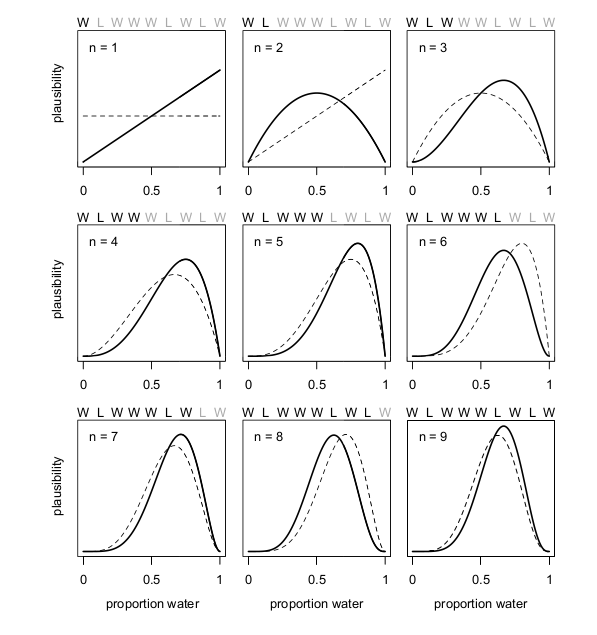
\includegraphics[scale=0.35]{pics/bayesUpdate.png}
\end{figure}

} 

\end{frame}



\begin{frame}{Calculating the Posterior}
\scriptsize{

\begin{itemize}

\item The posterior distribution encodes updated plausabilities (or beliefs) for all parameter values conditioned on the data.
\item As we have already seen, it can be obtained using the Bayes formula:

\begin{displaymath}
 f(p|W,L) = \frac{f(W,L|p)* f(p)}{f(W,L)}
\end{displaymath}

\item Where the denominator (evidence) makes sure that the posterior is a valid density function that integrates to one.

\item It is not always possible to compute the posterior analytically unless we constrain our prior to special forms that are easy to do mathematics with.

\item But bear in mind that in many of the interesting models in contemporary science we will need to approximate the posterior using computational techniques such as Markov Chain Montecarlo. 

\item This example is one the cases where the posterior can be found analytically as shown next.

\end{itemize}

} 


\end{frame}


\begin{frame}{Calculating the Posterior}
\scriptsize{

\begin{itemize}
\item The posterior of our globe model with binomial likelihood and uniform prior has a closed form which is a Beta distribution.
\begin{displaymath}
\mathbb{P}(p|W,L) = \text{Beta}(W+1 , L+1)
\end{displaymath}

\item This distribution is defined on the interval $[0, 1]$ and is parameterized by two positive shape parameters, denoted by $\alpha$ and $\beta$.

\item The Beta distribution is a continuous distribution on probabilities.

\begin{displaymath}
\text{Beta}(\alpha,\beta)=\frac{p^{\alpha-1}(1-p)^{\beta-1}}{\frac{\Gamma(\alpha)\Gamma(\beta)}{\Gamma(\alpha + \beta)}}
\end{displaymath}

\begin{figure}[h!]
	\centering
	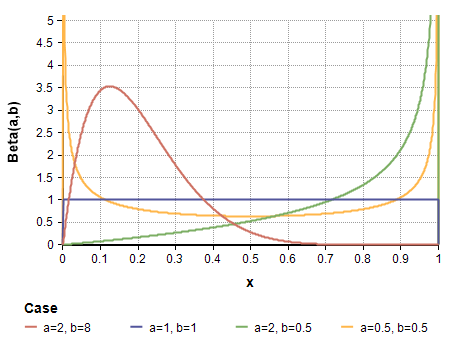
\includegraphics[scale=0.4]{pics/Beta(a,b).png}
\end{figure}

\end{itemize}

} 

\end{frame}




\begin{frame}{Calculating the Posterior}
\scriptsize{

\begin{itemize}
\item For any positive integer (such as W and L) the gamma function $\Gamma(n) = (n-1)!$

\item Hence, \begin{displaymath}
\text{Beta}(W+1 , L+1) = \frac{p^W(1-p)^L}{\frac{\Gamma(W+1)\Gamma(L+1)}{\Gamma(W+1 + L+1)}} = \frac{p^W(1-p)^L}{\frac{W!L!}{(W+L)!}} = \frac{(W+L)!}{W!L!}p^W(1-p)^L
\end{displaymath}

\item This surprisingly looks identical to the binomial distribution.

\item This is because both distributions are very similar. The binomial distribution models the number of successes (W) and the beta distribution models the probability $p$ of success. 


\item Let's build our posterior from the likelihood and the prior:
\begin{displaymath}
f(p|W,L) = \frac{f(W,L|p)*f(p)}{f(W,L)} = \frac{f(W,L|p)*f(p)}{\int_0^1f(W,L|p)*f(p)dp} 
\end{displaymath}

\end{itemize}

} 

\end{frame}



\begin{frame}{Calculating the Posterior}
\scriptsize{

\begin{itemize}


\item Since $f(p)=1$ (uniform prior) we have that

\begin{displaymath}
f(p|W,L) = \frac{f(W,L|p)}{\int_0^1f(W,L|p)dp} 
\end{displaymath}

\item The integral of the denominator is equal to 1 (essentially we are integrating a Beta distribution over its complete space of p):

\begin{figure}[h!]
	\centering
	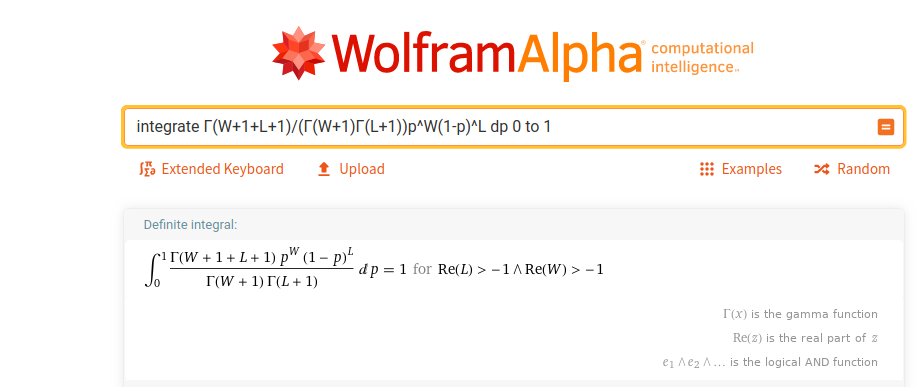
\includegraphics[scale=0.25]{pics/wolphram.png}
\end{figure}

\item So, we get 

\begin{displaymath}
f(p|W,L) =  \frac{(W+L)!}{W!L!}p^W(1-p)^L = \text{Beta}(W+1 , L+1) 
\end{displaymath}


\end{itemize}

} 

\end{frame}


\begin{frame}{Calculating the Posterior}
\scriptsize{

\begin{itemize}


\item So, in our globe tossing model $(W=6,L=3)$ we can calculate the posterior distribution analytically 

\begin{displaymath}
f(p|W=6,L=3) =  \text{Beta}(7,4) 
\end{displaymath}


\begin{figure}[h!]
	\centering
	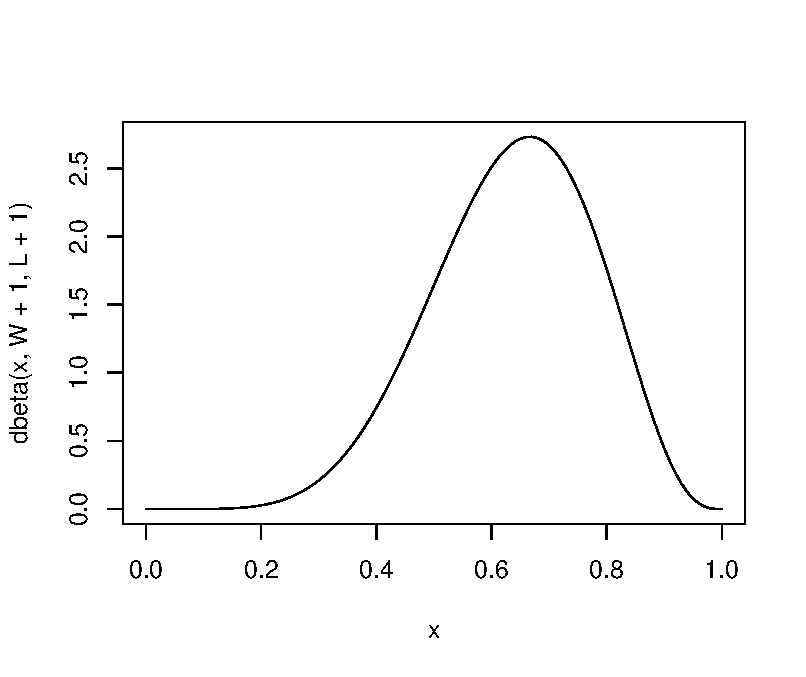
\includegraphics[scale=0.55]{pics/beta(7,4).pdf}
\end{figure}



\end{itemize}

} 

\end{frame}



\begin{frame}{Beta Prior}
\scriptsize{

\begin{itemize}

\item We could calculate the posterior analytically because a property called \textbf{conjugate priors}.

\item First of all, we must understand the Beta distribution is very flexible and can model a uniform distributions by setting $\alpha$ and $\beta$ to 1,  Beta(1,1)=Uniform

\item We can change now our prior to a more general one using a Beta distribution $f(p)=$Beta($\alpha$, $\beta$).

\item Now we can consider values of $\alpha$, $\beta$ that are more in line with our prior beliefs.

\item The nice thing here is that when the prior follows a Beta distribution  and the likelihood $f(W,L|p)$ a Binomial one, the posterior takes the form of another Beta distribution with parameters $(\alpha+W,\beta+L)$.

\item  The hyper-parameters of our Beta prior $\alpha$ and $\beta$  can be seen as ``pseudo-counts'' of successes and failures before collecting the data.  

\item This shows that our previous result for the uniform prior was a special case of this property.

\end{itemize}

} 

\end{frame}



\begin{frame}{Conjugate Priors}
\scriptsize{

\begin{itemize}
\item The Beta distribution is conjugate distribution to binomial distribution, which means that the posterior distribution in the same probability distribution family as the prior.

\item In simple words there are some families of conjugate distributions that can be used to calculate posterior distributions analytically.

\item A very complete table of conjugate distributions is given in \url{https://en.wikipedia.org/wiki/Conjugate_prior}.

\item In essence, conjugate priors constrain our choice of prior to special forms that are easy to do mathematics with.

\item However, there are numerical techniques that allow us to accommodate any prior that is most useful for our inference problem, such as Markov Chain Monte Carlo (MCMC).

\end{itemize}

} 

\end{frame}





\begin{frame}{Subjective Bayesian approach}
\scriptsize{

\begin{itemize}
\item Priors are engineering assumptions, chosen to help the machine learn.
\item They are also  scientific assumptions, chosen to reflect what we know about a phenomenon.
\item \textbf{Subjective Bayesian approach}:  a school of Bayesian inference that emphasizes choosing priors based upon the personal beliefs of the analyst. 
\item This subjective Bayesian approach is rare in the sciences.
\item The prior is considered to be just part of the model.
\item It should be chosen, evaluated, and revised just like all of the other components of the model.
\item The following diagram shows the effect of changing the prior in the globe tossing example.




\end{itemize}

} 

\end{frame}

\begin{frame}{Different Priors}
\scriptsize{

\begin{figure}[h!]
	\centering
	\includegraphics[scale=0.285]{pics/priorsGlobe.png}
\end{figure}
 
Top: A flat prior constructs a posterior that is simply
proportional to the likelihood. Middle: A step prior, assigning zero probability to all values less than 0.5, results in a truncated posterior. \\ Bottom: A peaked prior that shifts and skews the posterior, relative to the likelihood.
} 

\end{frame}



\begin{frame}{Motors}
\scriptsize{

\begin{itemize}
\item In many interesting models in contemporary science the posterior cannot be calculated analytically, no matter your
skill in mathematics.

\item Below are some numerical techniques for approximating the mathematics that follows from the definition of the posterior.

\begin{enumerate}
 \item Grid approximation
 \item Laplace approximation
 \item Markov chain Monte Carlo (MCMC)
 \item Variational Inference\footnote{Beyond the scope of this course.}
\end{enumerate}

\end{itemize}



} 
\end{frame}



\begin{frame}{Grid Approximation}
\scriptsize{

\begin{itemize}

\item Idea: consider only a finite grid of parameter values, and evaluate the posterior for all these points.


\item This approach scales very poorly, as the number of parameters increases.


\item It is mainly useful as a pedagogical tool, since learning it forces you to really understand the nature of Bayesian updating.


\end{itemize}

\begin{block}{Process}
\begin{enumerate}

  \item Define the grid. This means you decide how many points to use in estimating the posterior, and then you make a list of the parameter values on the grid.
\item Compute the value of the prior at each parameter value on the grid.
\item Compute the likelihood at each parameter value.
\item Compute the unstandardized posterior at each parameter value, by multiplying the prior by the likelihood.
\item  Finally, standardize the posterior, by dividing each value by the sum of all values.
\end{enumerate}
\end{block}

} 


\end{frame}

\begin{frame}[fragile]{Grid Approximation}
\begin{scriptsize}
 \begin{verbatim}
# define grid
p_grid <- seq( from=0 , to=1 , length.out=20 )
# define prior
prior <- rep( 1 , 20 )
# compute likelihood at each value in grid
likelihood <- dbinom( 6 , size=9 , prob=p_grid )
# compute product of likelihood and prior
unstd.posterior <- likelihood * prior
# standardize the posterior, so it sums to 1
posterior <- unstd.posterior / sum(unstd.posterior)
plot( p_grid , posterior,type="b",
xlab="probability of water",ylab="posterior probability")
mtext("20 points")
\end{verbatim}
\end{scriptsize}


\end{frame}


\begin{frame}{Grid Approximation}

\begin{figure}[h!]
	\centering
	\includegraphics[scale=0.4]{pics/grid.png}
\end{figure}


\end{frame}



\begin{frame}{Laplace Approximation}
\scriptsize{

\begin{itemize}
\item Under quite general conditions, the region near the peak of the posterior distribution will be nearly Gaussian in shape.
\item Idea: approximate the posterior distribution by a Gaussian distribution.
\item Gaussians are convenient because can be completely described by two parameters: $\mu$ and $\sigma$. 
\item The Laplace approximation is also called ``quadratic approximation'' because the logarithm of
a Gaussian distribution forms a parabola. 
\item A a parabola is a quadratic function.
\item Laplace approximation essentially represents any log-posterior with a parabola.
\end{itemize}


\begin{block}{Process}
\begin{enumerate}
  \item Maximum a Posteriori (MAP): Find the posterior mode using some optimization algorithm, a procedure that virtually “climbs” the posterior distribution.
  \item Once you find the peak of the posterior, you must estimate the curvature near the
peak.
\end{enumerate}
\end{block}


} 

\end{frame}



\begin{frame}[fragile]{Laplace Approximation}



\begin{scriptsize}

\begin{itemize}
 \item Laplace approximation is implemented in function \textbf{quap} from the \textbf{rethinking} R package.
 
 \item This package  will be used extensively in the remainder of this course.
 
 \item Installation instructions: \url{https://github.com/rmcelreath/rethinking}.
 
\end{itemize}
 \begin{verbatim}
library(rethinking)
globe.qa <- quap(
  alist(
    W ~ dbinom( W+L ,p) , # binomial likelihood
    p ~ dunif(0,1)   # uniform prior
  ) ,
  data=list(W=6,L=3) )

  # display summary of quadratic approximation
> precis( globe.qa )
  mean   sd 5.5% 94.5%
p 0.67 0.16 0.42  0.92

\end{verbatim}
Assuming the posterior is Gaussian, it is maximized at 0.67, and its standard deviation is 0.16.
\end{scriptsize}


\end{frame}



\begin{frame}{Laplace Approximation}
\scriptsize{

\begin{figure}[h!]
	\centering
	\includegraphics[scale=0.3]{pics/quadratic.png}
\end{figure}
 
\begin{itemize}
 \item Blue Curve: the exact posterior distribution. 
 \item Black Curve: the Laplace approximation.
 \item Left: The globe tossing data with n = 9 tosses and w = 6 waters.
 \item Middle: Double the amount of data, with the same fraction of water, n = 18 and w = 12.
 \item Right: Four times as much data, n = 36 and w = 24.
\end{itemize}


} 

\end{frame}


\begin{frame}{Maximum a Posteriori and Maximum Likelihood}
\scriptsize{

\begin{itemize}
\item The Laplace approximation, either with a uniform prior or with a lot of data, is often equivalent to a maximum likelihood estimate (MLE) and its standard error.
\item This is because maximum a posteriori with a uniform prior is equivalent to maximum likelihood estimation.
\item By using a uniform prior, our posterior is essentially the likelihood multiplied by a constant, so it makes sense that the maximum value of the posterior and the likelihood are the same.
\item More info: \url{https://wiseodd.github.io/techblog/2017/01/01/mle-vs-map/}.
\item This helps re-interpret many non-Bayesian models in Bayesian terms.
\end{itemize}


} 
\end{frame}



\begin{frame}{Markov Chain Monte Carlo}
\scriptsize{

\begin{itemize}
\item There are lots of important model types, like multilevel (mixed-effects) models, where Laplace approximation doesn't work.
\item Such models may have hundreds or thousands or tens-of-thousands of parameters so we can't use Grid approximation either.
\item Multilevel models do not always allow us to write down a single, unified function for the posterior distribution.
\item This means that the function to maximize (when finding the MAP) is not known, but must be computed in pieces. 
\item As a result, various counterintuitive model fitting techniques have arisen. 
\item The most popular of these is Markov chain Monte Carlo (MCMC).
\end{itemize}


} 
\end{frame}


\begin{frame}{Markov Chain Monte Carlo}
\scriptsize{

\begin{itemize}
\item Instead of attempting to compute or approximate the posterior distribution directly, MCMC techniques merely draw samples from the posterior.
\item You end up with a collection of parameter values, and the frequencies of these values correspond to the posterior plausibilities.
\item You can then build a picture of the posterior from the histogram of these samples.
We nearly always work directly with these samples, rather than first constructing some
mathematical estimate from them.
\item It is fair to say that MCMC is largely responsible for the insurgence of Bayesian data analysis that began in the 1990s. 
\item While MCMC is older than the 1990s, affordable computer power is not, so we must also thank the engineers.
\item Probabilistic programming: environments for designing Bayesian models and performing inference using numerical techniques (e.g., STAN, Pyro).
\end{itemize}


} 
\end{frame}



\begin{frame}{Conclusions}
\scriptsize{

\begin{itemize}
\item The target of inference in Bayesian inference is a posterior probability distribution.\item Posterior probabilities state the relative numbers of ways each conjectured cause of the data could have produced the data. 
\item These relative numbers indicate plausibilities of the different conjectures.
\item These plausibilities are updated in light of observations through Bayesian updating.
\item Bayesian models are fit to data using numerical techniques.
\item Each method imposes different trade-offs.

\end{itemize}


} 
\end{frame}


%%%%%%%%%%%%%%%%%%%%%%%%%%%
\begin{frame}[allowframebreaks]\scriptsize
\frametitle{References}
\bibliography{bio}
\bibliographystyle{apalike}
%\bibliographystyle{flexbib}
\end{frame}  









%%%%%%%%%%%%%%%%%%%%%%%%%%%

\end{document}
